\documentclass{article}
\usepackage{parskip}
\usepackage{indentfirst}
\setlength{\parindent}{1cm}
\renewcommand{\baselinestretch}{1.4}

\usepackage{graphicx}
\usepackage{url}
\usepackage{enumitem}
\usepackage{adjustbox}

\usepackage{hyperref}
\hypersetup{
    colorlinks=true,
    linkcolor=red,
    filecolor=blue,      
    urlcolor=blue,
    citecolor=red
}
 
\usepackage[
    top    = 3cm,
    bottom = 2cm,
    left   = 2.8cm,
    right  = 2.8cm]{geometry}
\usepackage[utf8]{inputenc}

\usepackage{fancyhdr}
\pagestyle{fancy}
\renewcommand{\headrulewidth}{0pt}
\fancyhf{}
\lhead{PHYS3051}
\rhead{Desiree Vogt-Lee}
\cfoot{\thepage}

\title{Implementing the Klein Gordon Equation on a Quantum Computer}
\author{Desiree Vogt-Lee, 44354471}
\date{10 June, 2019}

\begin{document}
	\maketitle
	\begin{center}
	    All components of this project including code, Jupyter Notebooks, LaTeX files and images can be found in my \href{https://github.com/desireevl/PHYS3051}{Github repository}, please check this out for reference.
	\end{center}


\section{The Klein Gordon Equation}

motivation 

\section{Background}
\subsection{Quantum Computing}
Quantum computing is the melding together of quantum mechanics and classical computation. The computer chips used in quantum computers use the same fundamental components as that of their classical counterparts, however are pieced together in a way which allow quantum-bits, or qubits, to be used instead of bits. 

A fundamental flaw in the current design of quantum computers is the large amount of error that is created due to noise and decoherence, which increases with the number of qubits used. This severely limits the computation that can be performed with a negligable amount of error, as at some point, the current error correcting codes will have little effect. 

Many believe that quantum computation is the future. Due to the superposition and entanglement properties these qubits can possess, all sorts of optimisation and new algorithms can be created, which would have significant impact on many fields of technology. For example, modern cryptography is centered around the assumption that creating incredibly long numbers take current computers an impossibly long time to factorise. Using Shor's algorithm, a quantum computer would be able to factorise a number in polynomial time, exponentially faster than the best classical algorithm, and thus being able to break modern cryptography. \cite{minutephysics}

At present, this is all merely a premonition; as although there exists many quantum algorithms, the error is too great and the number of qubits too little to be able to use them.

\subsection{Gates}
To modify the state that a qubit is in, a gate or procession of gates can be applied to it. The quantum gates are similar to the logic gates present in classical computing, but work with the quantum nature of the qubit. To easily conceptualise the effect of a quantum gate, a geometric representation called the Bloch sphere is used, where the poles of the sphere represent the standard basis vectors $|0\rangle$ and $|1\rangle$.

\begin{figure}[!htb]
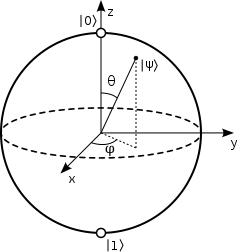
\includegraphics[scale=0.55]{../images/bloch_sphere}
  \centering
  \caption{Bloch Sphere \cite{blochsphere}}
\end{figure}

In classical computation, the NOT gate simply flips a given bit state: a 1 will be transformed to a 0 and vice versa. In quantum computing there is an equivalent X gate which when applied to a qubit in the $|0\rangle$ state, performs a rotation about the x axis on a Bloch sphere by $\pi$ radians resulting in the $|1\rangle$ state when measured (for more detailed explanation on the fundamental gates and terminology, please see my \href{https://desireevl.github.io/archive/2019/04/03/quantum-intro.html}{blog post}).

Here I will briefly explain the gates that will be used to create the circuit that implements the Klein Gordon equation (minus those explained in my blog post):
\newline

\begin{itemize}[labelindent=1.5em,labelsep=0.9cm,leftmargin=*]
	\item\adjustbox{valign=t}{
\includegraphics[width=0.7cm]{../images/t_gate}} {} {} {} {}  T: performs a $\frac{\pi}{4}$ rotation about the z axis, which is equivalent to a quarter of one Z gate operation. This gate acts on the phase of the qubit and is represented by the matrix: 
\[T=\left(\begin{array}{ll}{1} & {0} \\ {0} & {e^\frac{i\pi}{4}}\end{array}\right)\]
	\item\adjustbox{valign=t}{
\includegraphics[width=0.7cm]{../images/tdagger_gate}} {} {} {} {}  $T^\dagger$: simply the opposite of the T gate and applies a $-\frac{\pi}{4}$ rotation about the z axis \cite{qiskitt}.
	\item\adjustbox{valign=t}{
\includegraphics[width=0.7cm]{../images/u1_gate}} {} {} {} {}  $U_1$: performs a unitary rotation on the state vector where the continuous phase can be specified. It is represented by the following matrix and as can be seen, is of a similar to that of the T gate, suggesting that a $U_1(\frac{\pi}{4})$ gate is equivalent to a T gate.
	\[U_1(\lambda) = \left(\begin{array}{ll}{1} & {0} \\ {0} & {e^{i \lambda}}\end{array}\right)\]
	\item\adjustbox{valign=t}{
\includegraphics[width=0.7cm]{../images/u3_gate}}  {} {} {} {} $U_3$: used to perform arbitrary unitary operation, where the $\theta$, $\psi$ and $\lambda$ position of the vector on the Bloch sphere can be modified to any value. This is the most general form of a single qubit unitary operation and is represented in matrix form as \cite{qiskitu}:
	\[U=\left(\begin{array}{cc}{\cos (\theta / 2)} & {-e^{i \lambda} \sin (\theta / 2)} \\ {e^{i \phi} \sin (\theta / 2)} & {e^{i \lambda+i \phi} \cos (\theta / 2)}\end{array}\right)\]
    \item\adjustbox{valign=t}{
\includegraphics[width=0.7cm]{../images/measurement_gate}} {} {} {} {} Measurement: used at the end of the circuit to measure the outcome of the states in the z basis.
    \item\adjustbox{valign=t}{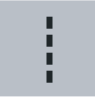
\includegraphics[width=0.25cm]{../images/barrier}} {} {} {} {} Barrier: directives which inform the complier not to optimise across barriers. They serve the purpose of keeping gates, especially measurement gates, in their place and are as well used as a visualisation tool to separate parts of the circuit.
\end{itemize}


\section{The Circuits}

In the code there is an option to choose to run the circuit on a real IBM quantum computer or the simulator.

\begin{figure}[!htb]
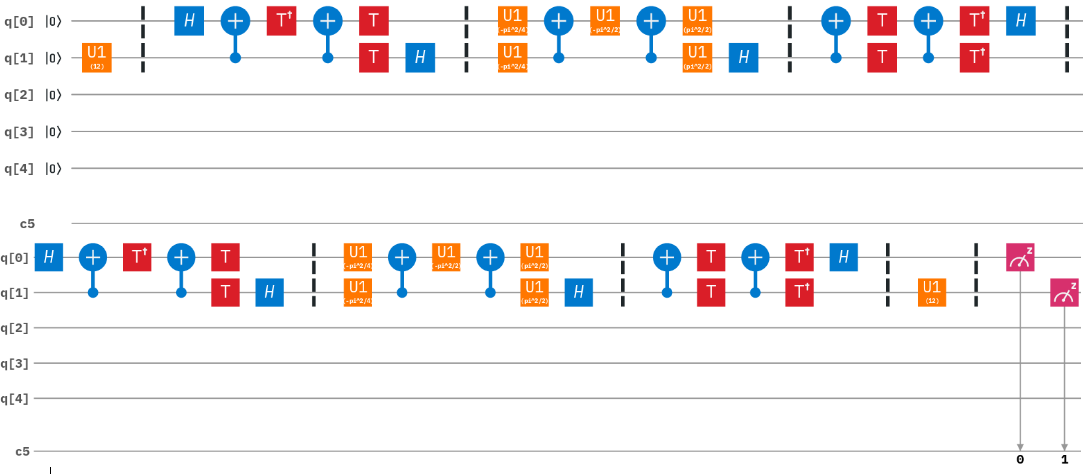
\includegraphics[scale=0.42]{../images/circuit1_colour}
  \centering
  \caption{Circuit 1}
\end{figure}

\begin{figure}[!htb]
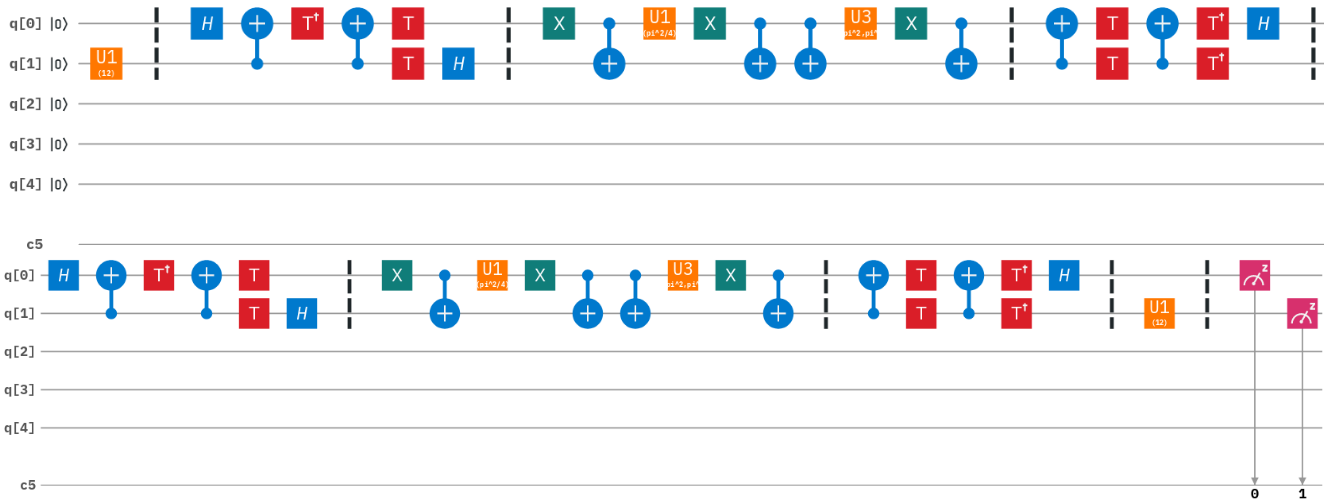
\includegraphics[scale=0.34]{../images/circuit2_colour}
  \centering
  \caption{Circuit 2}
\end{figure}
\subsection{Quantum Fourier Transform and its Inverse}


\section{Results}
\subsection{Kapil, M. et al. (2018) Results}

\subsection{My Results}


\bibliography{refs.bib}
\bibliographystyle{ieeetr}



\end{document}
